\documentclass[sigconf,anonymous,review,pbalance]{acmart}
\setcopyright{none}
\settopmatter{printacmref=false}
\renewcommand\footnotetextcopyrightpermission[1]{}
\acmConference[IAFM '26]{Workshop on Interpretability and Alignment of Financial Models}{November 2026}{Milan, Italy}
\acmYear{2026}
\title{Auditing Reward Alignment in Portfolio Learning: Exact Mismatch and Historical Calibration}
\author{Anonymous Author(s)}
\newcommand{\E}{\mathbb{E}}
\newcommand{\Var}{\operatorname{Var}}
\newcommand{\Cov}{\operatorname{Cov}}
\newcommand{\eq}{\mathrm{eq}}
\newtheorem{proposition}{Proposition}
\newtheorem{theorem}{Theorem}
\begin{document}
\begin{abstract}
Portfolio learners optimise specified rewards, which need not encode the investor's intended risk preferences. We study this alignment question separately from predictive skill and optimisation error. In an independent-return market, we derive the exact leading coefficient of the smallest policy discrepancy achievable by calibrating a quadratic wealth-increment reward. With nonzero interest, no common scalar penalty recovers the terminal mean--variance equilibrium over multiple dates. For constrained one-period allocation, an auxiliary-variable identity explains how second-moment calibration also changes turnover preferences; jointly scaling risk and cost coefficients preserves the fitted mean--variance optimum. We evaluate these statements using 432 monthly walk-forward decisions on ten US industry portfolios from 1990 to 2025. Joint calibration agrees with the reference to numerical precision across 17 settings; an adapted existing mean--variance policy iteration method also matches the primary reference. Unconstrained scalar calibration and a recent log-minus-variance reward adaptation retain measurable allocation differences. Exact alignment does not establish superior realised performance: paired bootstrap intervals for the principal historical mean--variance comparisons include zero. The contribution is an auditable distinction between financial preference alignment, learning accuracy and investment performance, supported by an exact mismatch result and a reproducible historical test.
\end{abstract}
\ccsdesc[500]{Computing methodologies~Reinforcement learning}
\ccsdesc[300]{Applied computing~Economics}
\keywords{portfolio allocation, reward alignment, mean--variance, reinforcement learning, transaction costs}
\maketitle

\section{Introduction}
Choosing a risk-sensitive reward is already an economic modelling decision. A learner that accurately maximises return minus a squared-return penalty can still implement different preferences from an investor who specified mean minus variance. The distinction is especially consequential when terminal objectives, intermediate rewards and transaction costs are expressed in different units.

Recent financial learning papers make the range of choices concrete. Jiang et al.\ \cite{jiang2025} optimise log return with a variance penalty and trading restrictions; their earlier work\ \cite{jiang2024} combines portfolio value, variance and trading costs. Simon et al.\ \cite{simon2026}, in contrast, directly optimise investor utility, including centred mean--variance preferences. AlphaPortfolio\ \cite{cong2026} supports whole-trajectory objectives through pathwise gradients. Thus the relevant question is not whether financial learning can optimise investor objectives. It is whether a particular reward implements a particular stated objective, and how to detect and repair discrepancies.

We contribute an exact best-in-family mismatch calculation for quadratic wealth-increment rewards, followed by a historical audit of constrained reward calibration. The former identifies an irreducible effect of interest over a fixed horizon. The latter gives an interpretable risk--cost coupling identity and tests it on past-only estimates from observed returns. The calibration identity follows established mean--variance auxiliary-variable methods; we include a corresponding prior-art baseline rather than presenting this identity as a new general optimisation algorithm.

Our method is to specify the financial reference, solve both the reference and reward-induced problems, measure their discrepancy on common states, and then assess finite-budget optimisation and realised performance separately. The result is useful even when it does not improve Sharpe: an allocator can verify whether a reward implements the preferences it was intended to implement.

\section{Related work and comparison design}
\paragraph{Objective-aware financial learning.}
Simon et al.\ \cite{simon2026} use deep parametric portfolio policies and US equity characteristics. Their Section 4.1, Eq.\ (17), specifies centred mean--variance utility; Section 3.6, Eqs.\ (14)--(16), treats turnover costs. Their Table 4 studies alternative preferences. This is a positive example of objective-aware learning, and our fitted covariance-MV reference shares this preference, not their architecture or empirical universe. Gollart and Okhrin\ \cite{gollart2025}, Section 4.2.1, Table 1, use zero intermediate rewards and terminal wealth utility, with modified DDPG tested against an analytical Heston--Nandi benchmark. Known-policy validation therefore predates our work. Chaouki et al.\ \cite{chaouki2020}, Section 3, likewise compare learned and known controls.

\paragraph{Additive rewards and trajectory objectives.}
Jiang et al.\ \cite{jiang2025}, Eq.\ (8), combine net log return with a variance penalty. Eq.\ (19) adds soft constraint penalties, and their DPG architecture uses CNN/WaveNet representations. Their Table 2 compares investment horizons across US and Canadian stock universes. We adapt the log-minus-variance preference to the same monthly estimates and hard simplex used by every comparator. We use a first-order turnover charge instead of their log cost factor. This isolates a reward comparison; it does not reproduce their architecture, data or reported performance. Jiang et al.\ \cite{jiang2024}, Eq.\ (4), penalise variance and trading costs around a portfolio-\emph{value} term, which cannot be silently equated to an excess-return increment. Their TD3/PPO/DDPG comparisons motivate studying risk and cost coefficients together, but are not reproduced here. Cong et al.\ \cite{cong2026}, Eqs.\ (19)--(20), optimise differentiable trajectory objectives, including a window Sharpe ratio. Such objectives are not presumed equivalent to terminal MV.

\paragraph{Mean--variance control and transformations.}
Precommitment\ \cite{ling2000} and equilibrium\ \cite{basak2010,dai2023} solve different time-inconsistent control questions. The distinction cannot be settled by a backtest ranking. Czichowsky\ \cite{czichowsky2013}, Lemma 3.2 of the inspected preprint, already gives a discrete continuation-covariance hedge. Bj\"ork et al.\ \cite{bkm2016}, Propositions 8.1 and 10.2 of the long 2016 preprint, give equivalent control objectives and terminal-unit variance penalisation. We do not claim either idea as new. Mean--variance policy iteration (MVPI)\ \cite{zhang2021} uses an auxiliary-variable transformation that contains our zero-interest calibration. Our specific theoretical increment is the exact local minimum discrepancy within the raw increment-reward family. We found no matching coefficient in these inspected sources; this is a scoped literature comparison, not a proof of priority.

\section{An exact test of terminal-objective alignment}
\subsection{Market, reference and discrepancy}
Consider independent excess returns $P_t\in\mathbb R^n$ with constant mean $m\ne0$ and positive definite covariance $\Sigma$. Wealth evolves as
\begin{equation}
 X_{t+1}=sX_t+P_t^\top u_t,\qquad X_0=x_0,
\end{equation}
with unrestricted risky dollar positions $u_t$ and constant gross risk-free return $s>0$. The terminal objective is $J=\E X_T-\varphi\Var X_T$, $\varphi>0$. The time-consistent equilibrium policy is
\begin{equation}
 u_t^\eq=\frac{\Sigma^{-1}m}{2\varphi H_t},\qquad H_t=s^{T-t-1}.
\end{equation}
It is not the initial-date precommitment maximiser. Define $M=\Sigma+mm^\top$, $d=M^{-1}m$, $\nu=m^\top d<1$ and $b=[2\varphi(1-\nu)]^{-1}$. The reward family is $r_t=\Delta X_t-\kappa(\Delta X_t)^2$, with one constant $\kappa>0$. Let $\pi^\kappa$ be its exact additive-reward optimum, and measure
\begin{equation}
 D^2=\sum_{t=0}^{T-1}\E_{\pi^\kappa}\|\pi^\kappa(t,X_t)-u_t^\eq\|^2.
\end{equation}
This is an occupancy-dependent discrepancy, not a symmetric policy metric.

\subsection{What scalar calibration cannot repair}
\begin{theorem}\label{th:mismatch}
For fixed $T\ge2$, as $s\to1$,
\begin{align}
 \min_{\kappa>0}D&=c_T|s-1|+O((s-1)^2),\\
 c_T&=\|d\|b\sqrt{\frac{T(T^2-1)}3+\frac{\nu(1-\nu)T(T-1)}2}.
\end{align}
At $s=1$ exact matching holds for $\kappa=\varphi(1-\nu)$. For $s\ne1$, $T\ge2$, exact matching along the surrogate occupancy is impossible.
\end{theorem}
\begin{proof}
Write the Bellman value $W_t(x)=p_tx^2+q_tx+c_t$, with $p_T=q_T=0$ and $g_t=\kappa(s-1)-sp_{t+1}$. Completing the square gives $u_t=\alpha_tx+\beta_t$ and
\begin{align}
 \alpha_t&=-\frac{dg_t}{\kappa-p_{t+1}},&
 \beta_t&=\frac{d(1+q_{t+1})}{2(\kappa-p_{t+1})},\\
 p_t&=\frac{\kappa p_{t+1}-(1-\nu)g_t^2}{\kappa-p_{t+1}},&
 1+q_t&=(1+q_{t+1})\left(s-\frac{\nu g_t}{\kappa-p_{t+1}}\right).
\end{align}
Induction gives $p_t\le0$, so the action Hessian is negative definite and these are global Markov optima. Set $e=s-1$, $h=(2\kappa)^{-1}$. The ratios $p_t/\kappa$ and $q_t$ are independent of $\kappa$, hence pathwise $X_t=L_t(e)x_0+hZ_t(e)$. Consequently $D^2=F(e,h)$ is exactly quadratic in $h$, with analytic coefficients near zero and $F(0,h)=T\|d\|^2(h-b)^2$. Its global minimiser is analytic and remains positive near zero.

Put $\kappa=\varphi(1-\nu)(1+we)$. The leading action difference is $de$ times
\[
 -X_t+b[(T-t-1)(2-\nu)-w].
\]
At $e=0$, $\E X_t=x_0+t\nu b$ and $\Var X_t=tb^2\nu(1-\nu)$. Minimisation yields $w^*=(T-1)(1-\nu)-x_0/b$. The centred means are $b(T-1-2t)$; summing their squares and variances gives the displayed $c_T^2$. Analyticity then gives the stated remainder after taking square roots.

Finally, matching at the first date forces a nonzero equilibrium action and positive subsequent wealth variance. At the final date the surrogate has slope $-d(s-1)$ whereas equilibrium is constant. Almost-sure equality is impossible when $s\ne1$.
\end{proof}
The coefficient grows as $T^{3/2}$ for large $T$, but the expansion is for fixed $T$; no uniform joint interest--horizon limit is claimed. The obstruction concerns this reward family, not all additive objectives.

\subsection{A reference-preserving reward}
Allow moments to vary by date while returns remain independent. Define $Y_t=H_tP_t^\top u_t$ and use
\begin{equation}\label{eq:design}
 r_t^{\rm design}=Y_t-\varphi(1-\nu_t)Y_t^2.
\end{equation}
The expected reward is strictly concave. Its maximiser is
\[u_t=\frac{\Sigma_t^{-1}m_t}{2\varphi H_t}.\] Future rewards admit state-independent maximisers, so backward induction recovers the equilibrium. This construction specialises established equivalent-objective ideas\ \cite{bkm2016}; it is not potential-based shaping preserving the original raw-reward policy. Dependent returns require continuation terms, so Eq.\ \eqref{eq:design} is not applied as a historical multiperiod theorem.

\begin{figure}[t]
\centering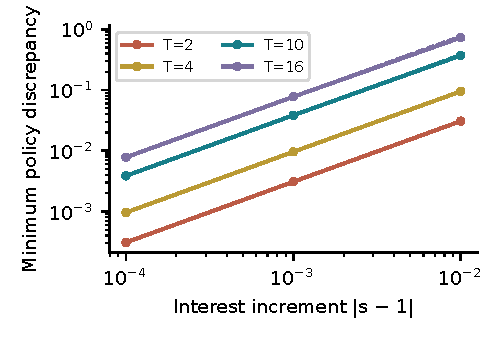
\includegraphics[width=\columnwidth]{figures/theory.pdf}
\caption{Exact minimum discrepancy (points and solid lines) and local prediction $c_T|s-1|$ (dashed lines). Here $x_0=\varphi=1$, $m=(.06,.04,.02)$, volatilities $(.18,.12,.08)$, and correlations $(\rho_{12},\rho_{13},\rho_{23})=(.30,-.10,.05)$. This concerns terminal equilibrium, not the fitted historical reference.}
\Description{Log-log plot comparing exact discrepancy with the local formula for four horizons.}
\label{fig:theory}
\end{figure}

\section{Constrained alignment with turnover costs}
Historical implementation adds constraints and costs. On a fixed past-only estimated state, let $C$ be the simplex, $p$ the pre-trade allocation and $c(u)=\|u-p\|_1$. Define the fitted one-period preference
\begin{equation}\label{eq:target}
 F(u)=m^\top u-\varphi u^\top\Sigma u-\lambda c(u),\quad u\in C.
\end{equation}
Its unique optimum $u^*$ is a \emph{fitted reference}, not the unknown true market optimum. This section does not extend Theorem~\ref{th:mismatch} to estimated or dependent markets.

\begin{proposition}\label{prop:joint}
Let $y^*=m^\top u^*$ and $A=1+2\varphi y^*>0$. The second-moment reward objective
\begin{equation}
 Q(u)=m^\top u-\frac{\varphi}{A}u^\top M u-\frac{\lambda}{A}c(u)
\end{equation}
has the same unique maximiser as $F$.
\end{proposition}
\begin{proof}
For all feasible $u$,
\begin{equation}\label{eq:identity}
 AQ(u)=F(u)-\varphi(m^\top u-y^*)^2+\varphi(y^*)^2.
\end{equation}
At $u^*$ the square vanishes and $F$ is maximal. Since $A>0$, the assertion follows.
\end{proof}
The identity remains a valid optimality argument on any feasible set with a global maximiser; convexity and positive definite covariance ensure uniqueness and computational tractability here. It follows the existing auxiliary-variable representation\ \cite{zhang2021}, not a new generic mean--variance transformation.

If only the risk coefficient is divided by $A$, while the cost coefficient stays $\lambda$, the right-hand side of Eq.\ \eqref{eq:identity} gains the extra term
\begin{equation}\label{eq:costdistortion}
 -2\varphi y^*\lambda c(u).
\end{equation}
When $y^*>0$, this increases the effective cost preference. It need not imply monotone realised turnover on the strategy's evolving path. The unconstrained formula $\varphi(1-\nu)$ likewise need not calibrate a constrained optimum.

The use of $u^*$ makes joint calibration an explicit reference-based certificate, not a faster way to compute an unknown reference. As a constructive prior-art comparator, we also alternate maximising
\begin{equation}
 (1+2\varphi y)m^\top u-\varphi u^\top Mu-\lambda c(u)
\end{equation}
and setting $y=m^\top u$. This is an adaptation of the MVPI mean auxiliary to the constrained one-period problem. Including the term $-\varphi y^2$ gives a jointly strictly concave objective, since its quadratic block has Schur complement $\Sigma\succ0$. Exact block updates converge to the same target. No advantage over exact MVPI is claimed.

\section{Historical study}
\subsection{Data and protocol}
We use Kenneth French's ten value-weighted US industry portfolio monthly total returns and the Fama--French risk-free series\ \cite{french}. The archived downloads have a recorded SHA-256 manifest. Estimation data start January 1970; evaluation covers January 1990--December 2025 (432 months). This is a retrospective study on the August 2026 revised vintage, not a point-in-time constituent dataset. Industry portfolios are research portfolios, not directly tradeable funds; their internal reconstruction costs are not included. The provider's CRSP processing and risk-free source changes also form part of this data vintage.

For month $t$, use only the previous 120 months of excess returns to estimate $m$ and the unbiased covariance, shrunk 10\% toward its diagonal. All strategies are long-only and fully invested. The primary settings are $\varphi=5$ and $\lambda=0.001$ (10 basis points per unit of L1 turnover). Pre-trade weights drift with realised gross asset returns. Net portfolio return uses the explicit first-order convention $u_t^\top R_t-\lambda\|u_t-p_t\|_1$, not a market-impact model or exact intramonth execution equation. These choices were recorded before inspecting strategy outcomes.

\subsection{Comparators and measurements}
We solve the covariance-MV target, raw second moment ($\kappa=\varphi$), unconstrained scalar calibration ($\kappa=\varphi(1-\nu)$), reference-based risk-only calibration, joint calibration, and MVPI adaptation. Equal weight and minimum variance provide conventional portfolio controls. Log utility and log-minus-variance adapt the reward preference in Jiang et al.\ \cite{jiang2025}; every method uses the same monthly data and feasible set. The comparison tests induced preferences under common estimates, not which published learning architecture is best.

For alignment, all methods face the target strategy's \emph{same pre-trade state}. We report Euclidean allocation distance and fitted regret $F(u^*)-F(u)$. Each strategy also follows its own pre-trade states for realised performance. This avoids conflating state divergence with the local reward comparison. Quadratic solutions have independent linear-programme first-order certificates; the largest saved common-state certificate is $4.27\times10^{-9}$ in objective units. The observed agreement of calibrated policies is considerably tighter than the acceptance tolerance.

Realised metrics are monthly excess-return MV, annualised excess Sharpe, return, volatility, turnover and drawdown. Uncertainty for paired MV differences uses 1,000 circular moving-block bootstrap resamples, blocks of 12 months, seed 8128. These intervals describe the observed strategy-return sequences, not full estimator-refitting or model-selection uncertainty. Robustness spans 17 prespecified combinations: $\varphi\in\{2,5,10\}$ and cost $\{0,10,25\}$ bp at the primary estimator, plus windows $\{60,120,240\}$ and covariance shrinkage $\{0,0.1,0.5\}$ at the primary preferences. The overlapping primary case is counted once.

\begin{table*}[t]
\centering
\caption{Primary historical comparison, 1990--2025. Distance and fitted regret use common states; realised metrics use each strategy's own path. Gap and MV score are monthly basis-point units. Calibration improves model alignment; the table does not establish superior investment performance.}
\label{tab:historical}
\begin{tabular}{lrrrr}\toprule
Method & Mean allocation distance & Fitted MV gap (bp) & Excess Sharpe & Realised MV (bp)\\\midrule
Target & 0.00000 & 0.0000 & 0.570 & -8.497 \\
Raw second moment & 0.00843 & 0.0148 & 0.573 & -7.182 \\
Unconstrained scalar & 0.00540 & 0.0043 & 0.568 & -8.882 \\
Risk-only calibration & 0.00510 & 0.0033 & 0.571 & -8.365 \\
Joint calibration & 0.00000 & 0.0000 & 0.570 & -8.497 \\
MVPI adaptation & 0.00000 & 0.0000 & 0.570 & -8.497 \\
Log minus variance & 0.01286 & 0.0287 & 0.572 & -7.123 \\
Log utility & 0.54848 & 39.7855 & 0.344 & -133.295 \\
Equal weight & 0.43495 & 46.2626 & 0.622 & -11.893 \\
Minimum variance & 0.23843 & 9.0252 & 0.645 & 5.274 \\
\bottomrule\end{tabular}

\end{table*}

\subsection{Results}
Table~\ref{tab:historical} shows that raw second-moment optimisation has mean allocation distance 0.00843. Unconstrained scalar calibration reduces this to 0.00540; reference-based risk-only calibration retains 0.00510. Joint calibration and MVPI agree with the fitted reference to numerical precision. The adapted log-minus-variance objective has distance 0.01286; log utility alone is much farther away. These numbers are numerically verified comparisons with a specified preference, not evidence that the other preferences are invalid.

Across all 17 settings, the largest mean joint-calibration distance is $1.54\times10^{-7}$; raw mean distances range from 0.00157 to 0.03682. Thus constraints and trading costs do not break the joint identity, while unconstrained scalar calibration is not a universal repair. Figure~\ref{fig:historical} relates alignment to historical outcomes, and Figure~\ref{fig:robust} gives robustness and uncertainty.

Joint calibration has realised monthly MV lower than raw by 1.315 bp, with 95\% interval $[-3.318,0.343]$ bp. Against scalar calibration the difference is 0.385 bp. Its interval is $[-0.570,1.351]$ bp. Against risk-only calibration the difference is $-0.131$ bp, with interval $[-0.889,0.634]$ bp. All include zero. Minimum variance has both a better realised MV score and higher Sharpe than the fitted target in the primary sample. This illustrates estimation risk: precise implementation of estimated preferences cannot guarantee the best realised allocation. Equal weight has higher Sharpe than the target but lower realised MV, so Sharpe ranking alone does not answer even the ex-post MV comparison.

\begin{figure*}[tp]
\centering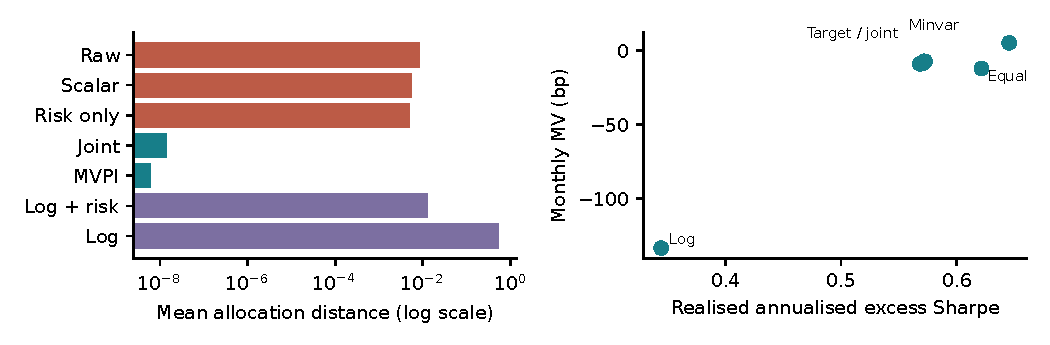
\includegraphics[width=.94\textwidth]{figures/historical.pdf}
\caption{Left: mean common-state allocation distance; the logarithmic axis exposes numerical agreement for joint calibration and MVPI. Right: realised Sharpe and monthly MV need not rank policies alike. Equal weight has higher Sharpe but lower MV than the fitted target.}
\Description{Allocation distances on the left and realised Sharpe versus mean-variance on the right.}
\label{fig:historical}
\end{figure*}
\begin{figure*}[tp]
\centering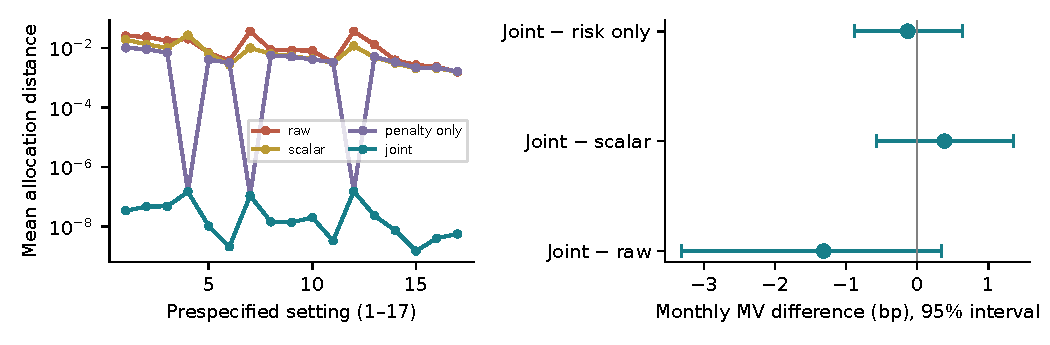
\includegraphics[width=.94\textwidth]{figures/robustness.pdf}
\caption{Left: alignment across the 17 prespecified settings, ordered by window, risk penalty, cost and shrinkage. Right: paired 12-month-block bootstrap intervals all include zero. Exact fitted alignment does not imply a statistically clear realised MV advantage.}
\Description{Seventeen-setting allocation-distance curves and three paired confidence intervals crossing zero.}
\label{fig:robust}
\end{figure*}

\subsection{Separating optimisation from reward design}
A finite-budget experiment assigns independent softmax policy logits to each of the 432 historical common states. Adam uses learning rate 0.05, initial logits $N(0,0.1^2)$, five matched seeds and 50, 250, 1,000 and 5,000 gradient steps. Each objective uses only its state's lagged estimates. This is a contextual direct-gradient optimisation diagnostic, not a predictive neural agent or reproduction of PPO, DDPG or the recent architectures.

Let $u_r$ maximise the specified reward and $\widehat u_r$ be the finite-budget allocation. We report the nonnegative own-reward optimisation gap separately from
\begin{align}
 F(u^*)-F(\widehat u_r)
 &= [F(u^*)-F(u_r)]\nonumber\\
 &\quad+[F(u_r)-F(\widehat u_r)].
\end{align}
The second bracket is a \emph{signed} target-value difference; it is not the own-reward optimisation gap. At 5,000 steps, mean own-reward optimisation gaps remain approximately $4\times10^{-6}$, exceeding the exact raw design gap of $1.48\times10^{-6}$. Thus finite-budget error can dominate the reward discrepancy. Figure~\ref{fig:learning} shows why these must be kept separate: improving the raw-reward optimiser does not remove its exact design gap. The target and joint reward have the same limiting optimum but can exhibit different finite-budget trajectories because their objective geometries differ.

\begin{figure*}[tp]
\centering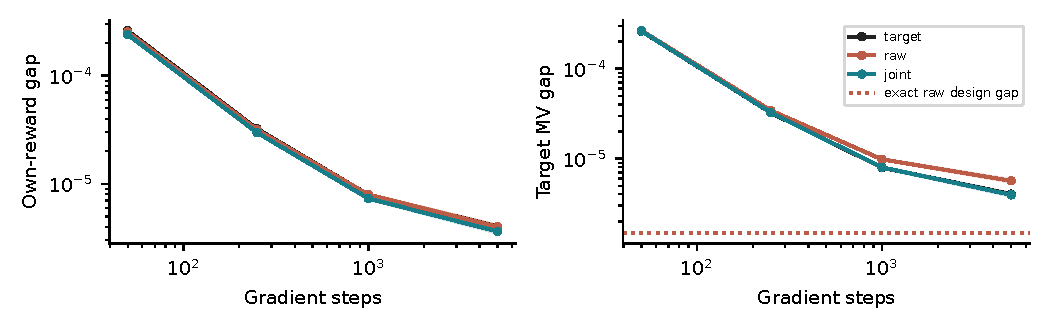
\includegraphics[width=.94\textwidth]{figures/learning.pdf}
\caption{Finite-budget softmax optimisation on historical fitted states. Lines are five-seed means, shading the seed range. Left uses each method's own reward; right uses the common MV target. The dotted line is the exact raw reward-design gap. This diagnostic measures optimisation accuracy, not generalisation.}
\Description{Own-reward and target gaps decline with gradient steps; the raw target gap remains above its design floor.}
\label{fig:learning}
\end{figure*}

\section{Implications and scope}
The analytical result is proved for independent returns and unrestricted dollar positions. The historical identity is proved for a fitted one-period problem with a positive calibration factor; its numerical application uses constrained allocations and lagged data. Neither result establishes a true historical terminal-MV equilibrium under dependence. The historical returns themselves need not be iid, but the rolling one-period reference does not identify their complete conditional law or continuation hedge.

The practical procedure is to state preferences before training, identify an appropriate reference, solve or approximate the reward optimum, and audit both on identical states. If a second-moment surrogate is used with turnover costs, Eq.\ \eqref{eq:costdistortion} identifies a concrete source of preference drift. A reference-based joint calibration or existing auxiliary-variable method removes that fitted discrepancy. Subsequent learning and historical performance remain separate empirical questions.

The strongest contribution is the exact fixed-horizon scalar-mismatch coefficient together with this explicit historical alignment audit. The work does not establish a new state-of-the-art trading algorithm. Its value for interpretable and aligned financial models is to make the economic meaning of a reward testable, including cases where successful optimisation or attractive Sharpe obscures the intended preference. Extending the exact audit to estimated dependent terminal equilibria and investable point-in-time assets remains a distinct research problem.

\clearpage
\bibliographystyle{ACM-Reference-Format}
\bibliography{references}
\end{document}
